\documentclass[10pt,journal,compsoc]{IEEEtran}

\usepackage{graphicx}
\usepackage{amsmath}
\usepackage{algorithm}
\usepackage{algorithmic}
\usepackage{array}
\usepackage{url}
\usepackage{hyperref}
\usepackage{subcaption}

\begin{document}

\title{Neural Implicit Functions: A Comparative Study of Implementation Approaches}

\author{Christian~Beneke}

\maketitle

\begin{abstract}
Neural Implicit Functions (NIFs) have emerged as a powerful approach for representing continuous functions in various domains, particularly for spatio-temporal data modeled by PDEs. This paper presents a comparative study of three different implementations of NIFs: an upstream reference implementation, a PyTorch-based approach, and a functional API design. We evaluate these implementations on both simple periodic and complex high-frequency wave functions, analyzing their performance, convergence characteristics, and implementation trade-offs. Our results demonstrate that while all implementations successfully model the target functions, they exhibit different strengths in terms of convergence speed, accuracy, and code maintainability. The functional API implementation shows superior performance for high-frequency cases, achieving up to 4x better loss values compared to the baseline.
\end{abstract}

\section{Introduction}
The representation and simulation of complex spatio-temporal phenomena, particularly those governed by partial differential equations (PDEs), remains a significant challenge in computational science \cite{neural_fields2022}. Traditional approaches often rely on discrete mesh representations, which can become computationally intractable for complex geometries or require adaptive meshing techniques. Neural Implicit Functions (NIFs) have emerged as a promising solution, offering a continuous, mesh-agnostic representation through neural networks \cite{nif2023}.

This paper focuses on the practical aspects of implementing NIFs, comparing different architectural approaches and their impact on performance and usability. We implement and analyze three distinct approaches:
\begin{itemize}
    \item An upstream reference implementation following traditional object-oriented principles
    \item A PyTorch-based implementation leveraging native framework features
    \item A functional API design emphasizing composability and clear data flow
\end{itemize}

\section{Background and Related Work}
\subsection{Neural Implicit Functions}
Neural Implicit Functions represent continuous functions through neural networks, typically combining two key components: a ShapeNet for encoding spatial complexity and a ParameterNet for modeling temporal and parametric dependencies \cite{nif2023}. This approach has shown promise in various applications, from computer graphics to scientific computing \cite{neural_fields2022}.

\subsection{HyperNetworks}
A key component of NIFs is the use of HyperNetworks \cite{hypernetworks2016}, which generate weights for target networks. We explore two main architectures:
\begin{itemize}
    \item ShortCut HyperNetwork: Utilizing direct skip connections for efficient parameter usage and faster convergence
    \item SIREN HyperNetwork: Employing sinusoidal activations for better frequency fitting and smooth representations \cite{siren2020}
\end{itemize}

\begin{figure}[t]
    \centering
    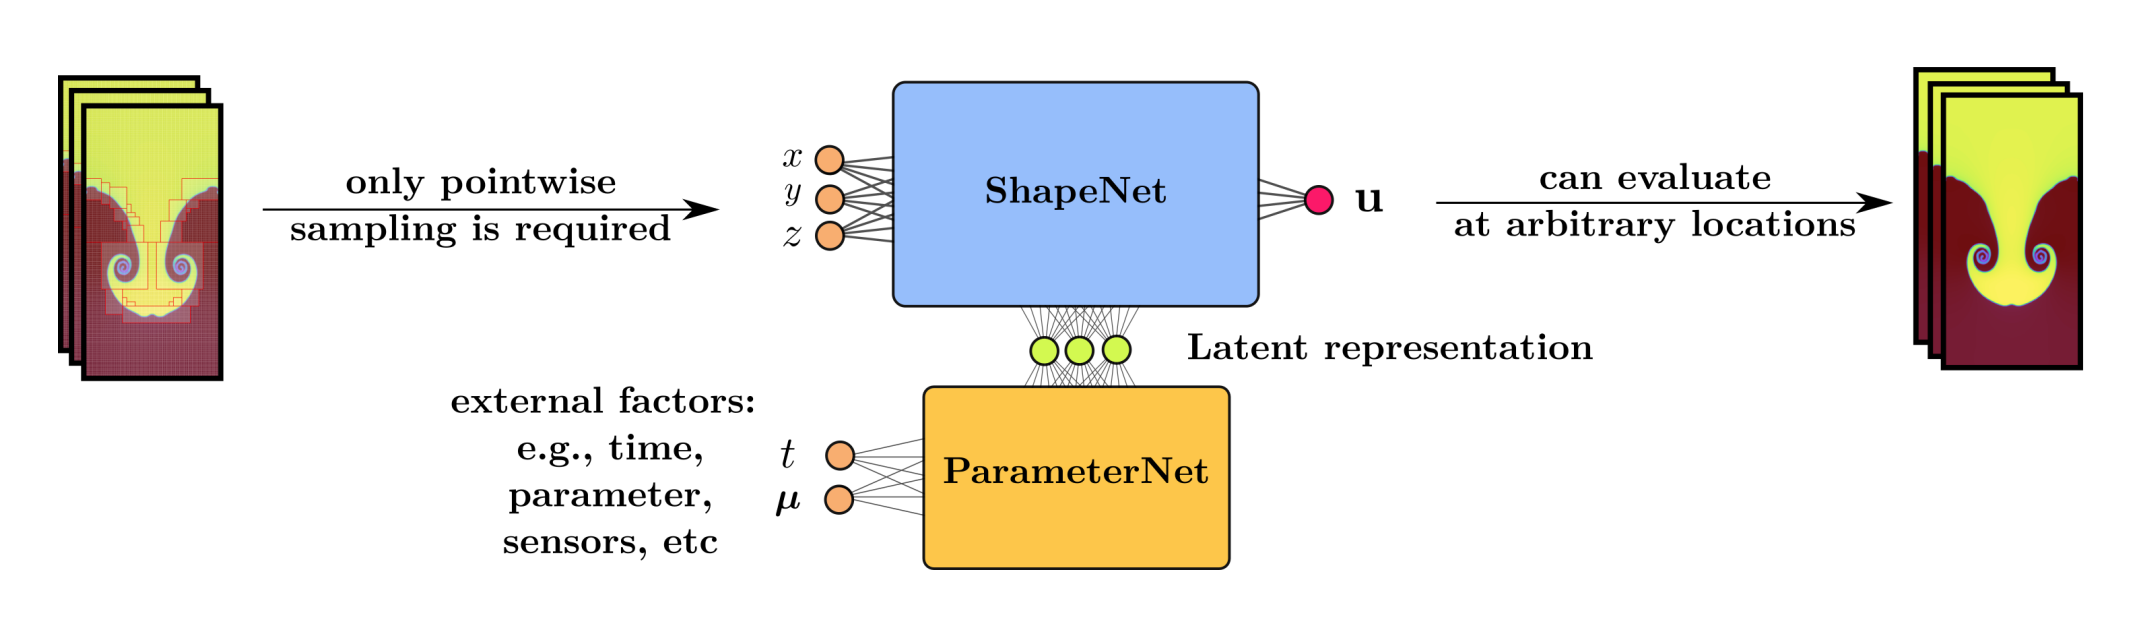
\includegraphics[width=0.8\linewidth]{hypernetwork_diagram}
    \caption{Architecture of the Neural Implicit Function with HyperNetwork. The HyperNetwork generates weights for the target network based on temporal parameters, while the target network processes spatial coordinates to produce the output.}
    \label{fig:architecture}
\end{figure}

\section{Methodology}
\subsection{Implementation Approaches}
We developed three distinct implementations of NIFs, each following different design philosophies:

\subsubsection{Upstream Implementation}
The reference implementation follows traditional object-oriented design principles, providing a baseline for comparison. This approach emphasizes code organization and maintainability through class hierarchies and clear separation of concerns.

\subsubsection{PyTorch Implementation}
Our PyTorch-based implementation leverages the framework's native features, particularly its automatic differentiation and tensor operations. This approach aims to balance performance with ease of use, taking advantage of PyTorch's ecosystem.

\subsubsection{Functional API}
The functional API implementation adopts a functional programming paradigm, emphasizing immutability and composability. This approach facilitates clearer data flow and easier testing, while potentially offering better optimization opportunities.

\section{Experimental Setup}
\subsection{Test Cases}
We evaluate our implementations on two distinct test cases, illustrated in Figure \ref{fig:test_cases}:

\begin{figure}[t]
    \centering
    \begin{subfigure}[b]{0.48\linewidth}
        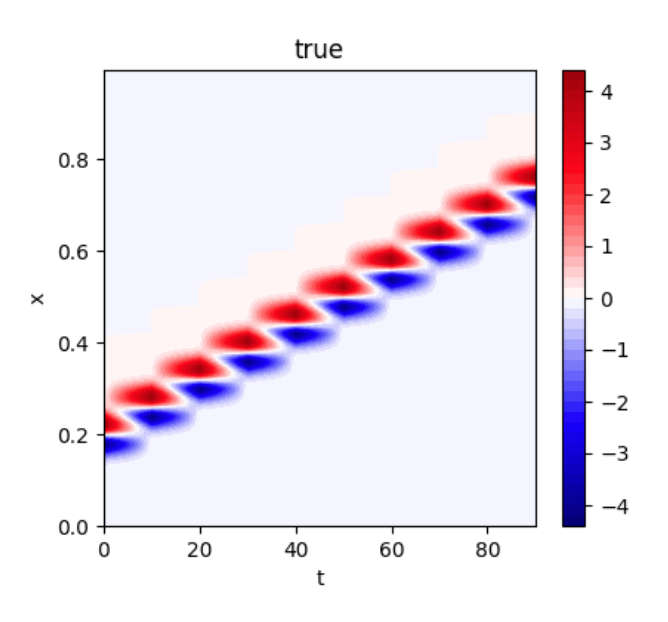
\includegraphics[width=\linewidth]{low_frequency}
        \caption{Low-frequency wave}
    \end{subfigure}
    \begin{subfigure}[b]{0.48\linewidth}
        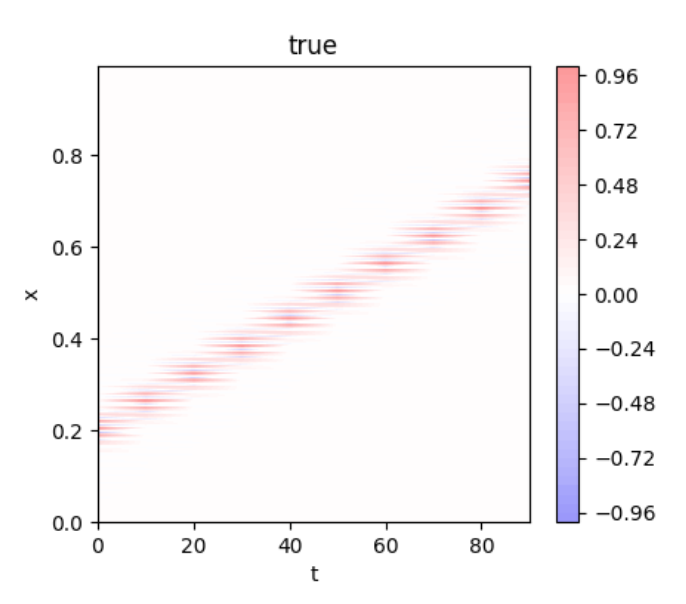
\includegraphics[width=\linewidth]{high_frequency}
        \caption{High-frequency wave}
    \end{subfigure}
    \caption{Test cases used for evaluation. (a) Simple periodic function serving as a baseline. (b) Complex wave function testing the model's capacity to capture high-frequency patterns.}
    \label{fig:test_cases}
\end{figure}

\subsection{Network Architectures}
Both test cases were evaluated using two different HyperNetwork architectures:
\begin{itemize}
    \item ShortCut HyperNetwork with direct skip connections
    \item SIREN HyperNetwork with sinusoidal activations
\end{itemize}

\section{Results and Discussion}
\subsection{Performance Analysis}
Our experiments reveal distinct performance characteristics across implementations, as shown in Figure \ref{fig:results}:

\begin{figure}[t]
    \centering
    \begin{subfigure}[b]{0.48\linewidth}
        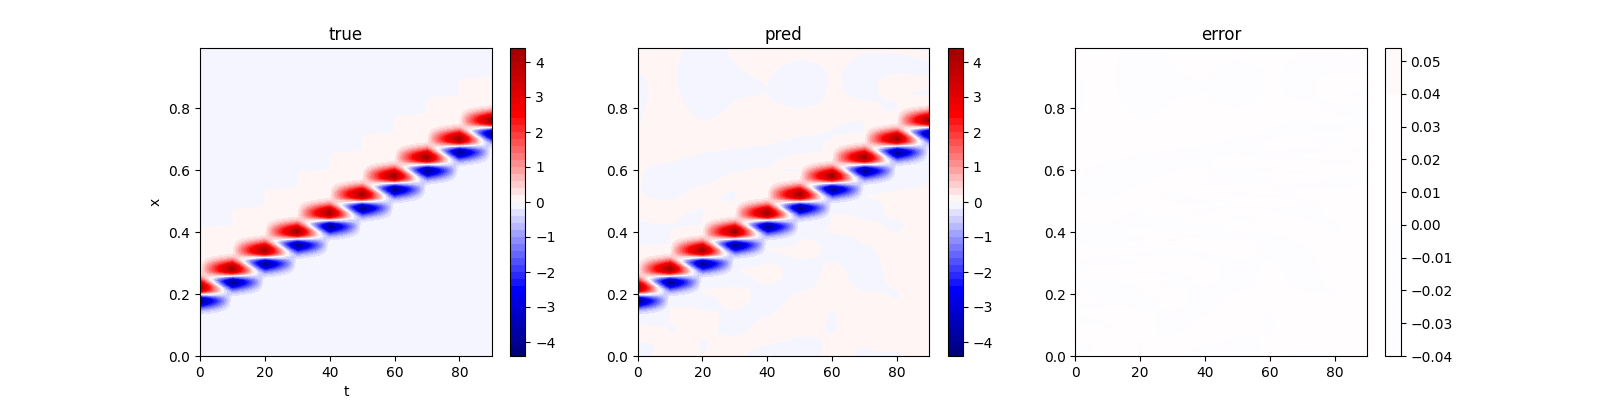
\includegraphics[width=\linewidth]{functional_vis_low}
        \caption{Low-frequency prediction}
    \end{subfigure}
    \begin{subfigure}[b]{0.48\linewidth}
        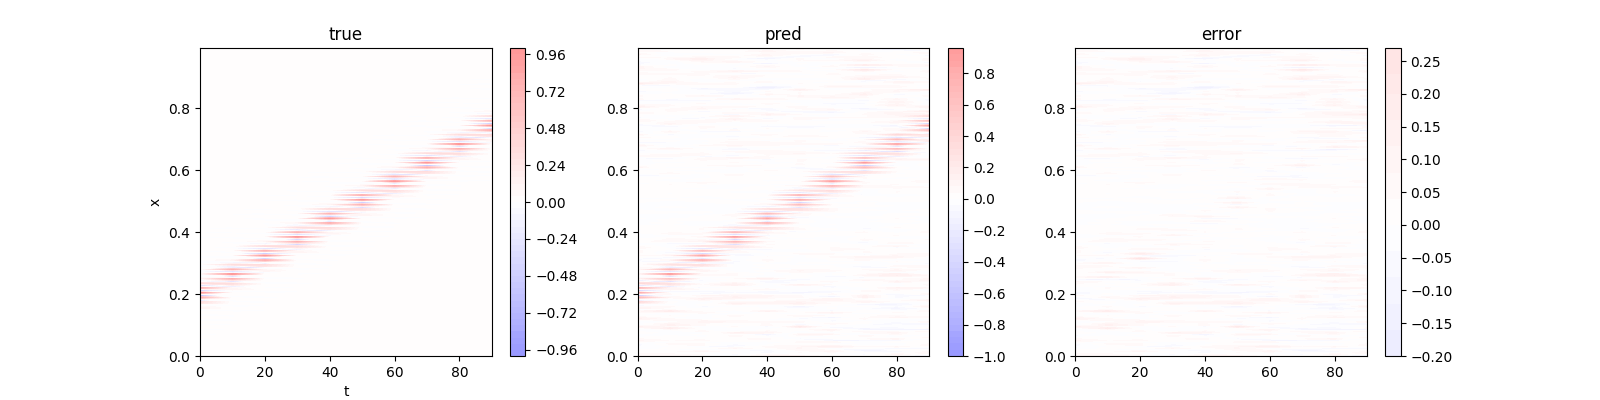
\includegraphics[width=\linewidth]{functional_vis_high}
        \caption{High-frequency prediction}
    \end{subfigure}
    
    \begin{subfigure}[b]{0.32\linewidth}
        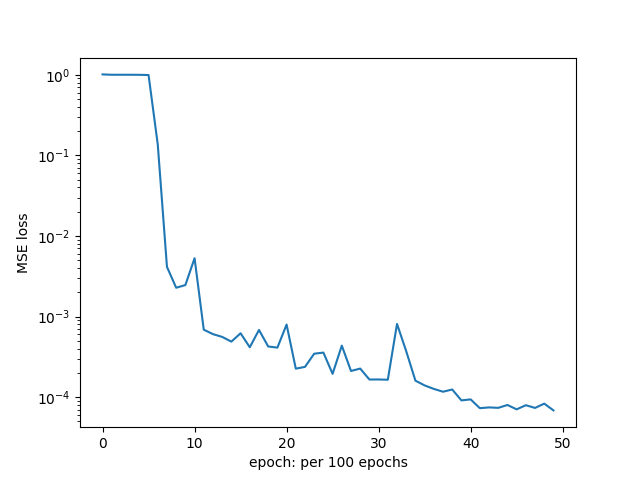
\includegraphics[width=\linewidth]{upstream_loss}
        \caption{Upstream loss}
    \end{subfigure}
    \begin{subfigure}[b]{0.32\linewidth}
        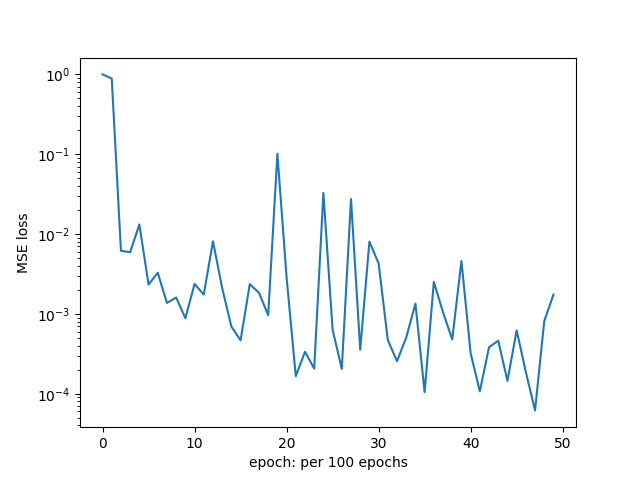
\includegraphics[width=\linewidth]{torch_loss}
        \caption{PyTorch loss}
    \end{subfigure}
    \begin{subfigure}[b]{0.32\linewidth}
        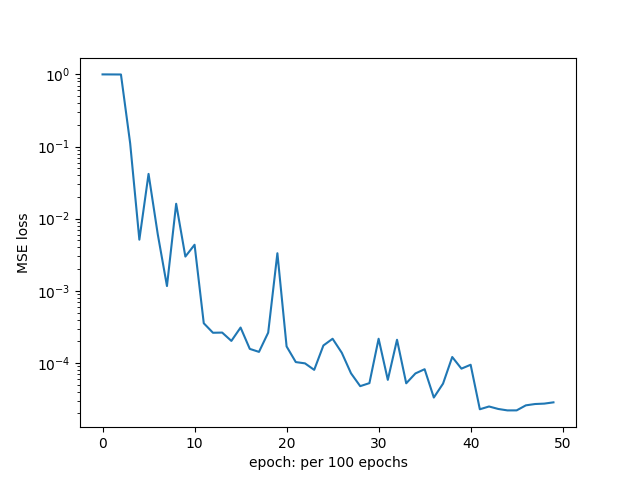
\includegraphics[width=\linewidth]{functional_loss_low}
        \caption{Functional API loss}
    \end{subfigure}
    \caption{Results comparison across implementations. (a,b) Visualization of predictions for both test cases using the functional API implementation. (c-e) Training loss curves for each implementation approach.}
    \label{fig:results}
\end{figure}

\begin{itemize}
    \item The upstream implementation achieves fast initial convergence with a best loss of 7.316e-05
    \item The functional API demonstrates superior performance on high-frequency cases, achieving a best loss of 2.198e-05
    \item The PyTorch implementation shows comparable performance to the upstream version (best loss: 6.178e-05) but with higher variance
\end{itemize}

\subsection{Implementation Trade-offs}
Each implementation approach presents distinct advantages and challenges:

\begin{itemize}
    \item The upstream implementation offers good baseline performance and clear code structure
    \item The PyTorch implementation provides excellent framework integration but shows more performance variance
    \item The functional API achieves the best numerical results but requires a different programming paradigm
\end{itemize}

\section{Conclusion}
This study demonstrates the successful implementation of Neural Implicit Functions across three different approaches, each with its own strengths and trade-offs. The functional API implementation shows particular promise for high-frequency cases, while the upstream and PyTorch implementations offer good baseline performance with different development advantages.

Future work could explore:
\begin{itemize}
    \item Additional network architectures for specific use cases
    \item Performance optimizations across implementations
    \item Extension to more complex spatio-temporal problems
\end{itemize}

\bibliographystyle{IEEEtran}
\bibliography{references}

\end{document}
